\documentclass[onesided]{article}\usepackage[]{graphicx}\usepackage[]{color}
% maxwidth is the original width if it is less than linewidth
% otherwise use linewidth (to make sure the graphics do not exceed the margin)
\makeatletter
\def\maxwidth{ %
  \ifdim\Gin@nat@width>\linewidth
    \linewidth
  \else
    \Gin@nat@width
  \fi
}
\makeatother

\definecolor{fgcolor}{rgb}{0.345, 0.345, 0.345}
\newcommand{\hlnum}[1]{\textcolor[rgb]{0.686,0.059,0.569}{#1}}%
\newcommand{\hlstr}[1]{\textcolor[rgb]{0.192,0.494,0.8}{#1}}%
\newcommand{\hlcom}[1]{\textcolor[rgb]{0.678,0.584,0.686}{\textit{#1}}}%
\newcommand{\hlopt}[1]{\textcolor[rgb]{0,0,0}{#1}}%
\newcommand{\hlstd}[1]{\textcolor[rgb]{0.345,0.345,0.345}{#1}}%
\newcommand{\hlkwa}[1]{\textcolor[rgb]{0.161,0.373,0.58}{\textbf{#1}}}%
\newcommand{\hlkwb}[1]{\textcolor[rgb]{0.69,0.353,0.396}{#1}}%
\newcommand{\hlkwc}[1]{\textcolor[rgb]{0.333,0.667,0.333}{#1}}%
\newcommand{\hlkwd}[1]{\textcolor[rgb]{0.737,0.353,0.396}{\textbf{#1}}}%
\let\hlipl\hlkwb

\usepackage{framed}
\makeatletter
\newenvironment{kframe}{%
 \def\at@end@of@kframe{}%
 \ifinner\ifhmode%
  \def\at@end@of@kframe{\end{minipage}}%
  \begin{minipage}{\columnwidth}%
 \fi\fi%
 \def\FrameCommand##1{\hskip\@totalleftmargin \hskip-\fboxsep
 \colorbox{shadecolor}{##1}\hskip-\fboxsep
     % There is no \\@totalrightmargin, so:
     \hskip-\linewidth \hskip-\@totalleftmargin \hskip\columnwidth}%
 \MakeFramed {\advance\hsize-\width
   \@totalleftmargin\z@ \linewidth\hsize
   \@setminipage}}%
 {\par\unskip\endMakeFramed%
 \at@end@of@kframe}
\makeatother

\definecolor{shadecolor}{rgb}{.97, .97, .97}
\definecolor{messagecolor}{rgb}{0, 0, 0}
\definecolor{warningcolor}{rgb}{1, 0, 1}
\definecolor{errorcolor}{rgb}{1, 0, 0}
\newenvironment{knitrout}{}{} % an empty environment to be redefined in TeX

\usepackage{alltt}
\usepackage[T1]{fontenc}
\linespread{1.5} % Line spacing - Palatino needs more space between lines
\usepackage{microtype} % Slightly tweak font spacing for aesthetics

\usepackage[hmarginratio=1:1,columnsep=20pt]{geometry} % Document margins
%\usepackage{multicol} % Used for the two-column layout of the document
\usepackage[hang, small,labelfont=bf,up,textfont=it,up]{caption} % Custom captions under/above floats in tables or figures
\usepackage{booktabs} % Horizontal rules in tables
\usepackage{float} % Required for tables and figures in the multi-column environment - they need to be placed in specific locations with the [H] (e.g. \begin{table}[H])

\usepackage{lettrine} % The lettrine is the first enlarged letter at the beginning of the text
\usepackage{paralist} % Used for the compactitem environment which makes bullet points with less space between them

% to ignore texts: good for thank messages and paper submissions.
      % \fbox{\phantom{This text will be invisible too, but a box will be printed arround it.}}

\usepackage{abstract} % Allows abstract customization
\renewcommand{\abstractnamefont}{\normalfont\bfseries} % Set the "Abstract" text to bold
%\renewcommand{\abstracttextfont}{\normalfont\small\itshape} % Set the abstract itself to small italic text

\usepackage[]{titlesec} % Allows customization of titles
\renewcommand\thesection{\Roman{section}} % Roman numerals for the sections
\renewcommand\thesubsection{\Roman{subsection}} % Roman numerals for subsections
\titleformat{\section}[block]{\large\scshape\centering}{\thesection.}{1em}{} % Change the look of the section titles
\titleformat{\subsection}[block]{\large}{\thesubsection.}{1em}{} % Change the look of the section titles

\usepackage{fancybox, fancyvrb, calc}
\usepackage[svgnames]{xcolor}
\usepackage{physics}
\usepackage{epigraph}
\usepackage{longtable}
\usepackage{pdflscape}
\usepackage{graphics}
\usepackage{pbox} % \pbox{20cm}{This is the first \\ cell}
\usepackage{amsfonts}
\usepackage{amsmath}
\usepackage{amssymb}
\usepackage{rotating}
\usepackage{paracol}
\usepackage{textcomp}
\usepackage[export]{adjustbox}
\usepackage{afterpage}
\usepackage{filecontents}
\usepackage{color}
\usepackage{latexsym}
\usepackage{lscape}       %\begin{landscape} and \end{landscape}
\usepackage{wasysym}
\usepackage{dashrule}
\usepackage{marvosym} % face package
\usepackage{framed}
\usepackage{tree-dvips}
\usepackage{pgffor}
\usepackage[]{authblk}
\usepackage{setspace}
\usepackage{array}
\usepackage[latin1]{inputenc}
\usepackage{hyperref}     %desactivar para link rojos
\usepackage{graphicx}
\usepackage{dcolumn} % for R tables
\usepackage{multirow} % For multirow in tables
\usepackage{pifont}
\usepackage{listings}
\usepackage{bm}




% hypothesis / theorem package begin
\usepackage{amsthm}
\usepackage{thmtools}
\declaretheoremstyle[
spaceabove=6pt, spacebelow=6pt,
headfont=\normalfont\bfseries,
notefont=\mdseries, notebraces={(}{)},
bodyfont=\normalfont,
postheadspace=0.6em,
headpunct=:
]{mystyle}
\declaretheorem[style=mystyle, name=Hypothesis, preheadhook={\renewcommand{\thehyp}{H\textsubscript{\arabic{hyp}}}}]{hyp}

\usepackage{cleveref}
\crefname{hyp}{hypothesis}{hypotheses}
\Crefname{hyp}{Hypothesis}{Hypotheses}
% hypothesis / theorem package end


%----------------------------------------------------------------------------------------
% Other ADDS-ON
%----------------------------------------------------------------------------------------

% independence symbol \independent
\newcommand\independent{\protect\mathpalette{\protect\independenT}{\perp}}
\def\independenT#1#2{\mathrel{\rlap{$#1#2$}\mkern2mu{#1#2}}}







\hypersetup{
    bookmarks=true,         % show bookmarks bar?
    unicode=false,          % non-Latin characters in Acrobat's bookmarks
    pdftoolbar=true,        % show Acrobat's toolbar?
    pdfmenubar=true,        % show Acrobat's menu?
    pdffitwindow=true,     % window fit to page when opened
    pdfstartview={FitH},    % fits the width of the page to the window
    pdftitle={My title},    % title
    pdfauthor={Author},     % author
    pdfsubject={Subject},   % subject of the document
    pdfcreator={Creator},   % creator of the document
    pdfproducer={Producer}, % producer of the document
    pdfkeywords={keyword1} {key2} {key3}, % list of keywords
    pdfnewwindow=true,      % links in new window
    colorlinks=true,       % false: boxed links; true: colored links
    linkcolor=ForestGreen,          % color of internal links (change box color with linkbordercolor)
    citecolor=ForestGreen,        % color of links to bibliography
    filecolor=ForestGreen,      % color of file links
    urlcolor=ForestGreen           % color of external links
}

%\usepackage[nodayofweek,level]{datetime} % to have date within text

\newcommand{\LETT}[3][]{\lettrine[lines=4,loversize=.2,#1]{\smash{#2}}{#3}} % letrine customization



% comments on margin
  % Select what to do with todonotes: 
  % \usepackage[disable]{todonotes} % notes not showed
  \usepackage[draft]{todonotes}   % notes showed
  % usage: \todo{This is a note at margin}

\usepackage{cooltooltips}

%%% bib begin
\usepackage[american]{babel}
\usepackage{csquotes}
\usepackage[backend=biber,style=authoryear,dashed=false,doi=false,isbn=false,url=false,arxiv=false]{biblatex}
%\DeclareLanguageMapping{american}{american-apa}
\addbibresource{/Users/hectorbahamonde/Bibliografia_PoliSci/library.bib} 
\addbibresource{/Users/hectorbahamonde/Bibliografia_PoliSci/Bahamonde_BibTex2013.bib} 

% USAGES
%% use \textcite to cite normal
%% \parencite to cite in parentheses
%% \footcite to cite in footnote
%% the default can be modified in autocite=FOO, footnote, for ex. 
%%% bib end

\usepackage{fancyhdr} % Headers and footers
\pagestyle{fancy} % All pages have headers and footers
\fancyhead{} % Blank out the default header
\fancyfoot{} % Blank out the default footer
\fancyhead[C]{MLE para Outcomes Ordenados: Ordered Logit/Probit} % Custom header text
\fancyfoot[RO,LE]{\thepage} % Custom footer text
\IfFileExists{upquote.sty}{\usepackage{upquote}}{}
\begin{document}
% DOCUMENT ID
%----------------------------------------------------------------------------------------
%	CONTENT
%----------------------------------------------------------------------------------------

%\graphicspath{
%{/Users/hectorbahamonde/RU/Term5/Experiments_Redlawsk/Experiment/Data/}
%}



%%%%%%%%%%%%%%%%%%%%%%%%%%%%%%%%%%%%%%%%%%%%%%
% begin knitr stuff


%%%%%%%%%%%%%%%%%%%%%%%%%%%%%%%%%%%%%%%%%%%%%%





\hspace{-5mm}{\bf Profesor}: H\'ector Bahamonde, PhD.\\
\texttt{e:}\href{mailto:hector.bahamonde@uoh.cl}{\texttt{hector.bahamonde@uoh.cl}}\\
\texttt{w:}\href{http://www.hectorbahamonde.com}{\texttt{www.hectorbahamonde.com}}\\
{\bf Curso}: MLE.\\
\hspace{-5mm}{\bf TA}: Gonzalo Barr\'ia.

\section{Outcomes Ordenados: Ordered Logit/Probit}


Los \emph{outcomes ordenados} son aquellos donde la variable dependiente es categ\'orica, pero representa cierto orden. Uno de los ejemplos m\'as t\'ipicos, es el de la \emph{escala de Likert}. La escala de Likert se utiliza para caracterizar, por ejemplo, niveles de aprobaci\'on/desaprobaci\'on de candidatos, pol\'iticas p\'ublicas, etc. La escala de Likert tiene en general cinco niveles de respuesta: \emph{muy de acuerdo}, \emph{acuerdo}, \emph{neutral}, \emph{desacuerdo}, \emph{muy en desacuerdo}. 

Lamentablemente, analistas insisten en analizar estas variables dependientes intervalares usando m\'etodos lineales OLS \parencite[115]{Long:1997wv}. Esto genera sesgos en los an\'alisis porque asume que los intervalos num\'ericos entre cada categor\'ia son constantes. Es decir, la distancia (num\'erica) que existe entre  \emph{muy de acuerdo} y \emph{acuerdo} es la misma que \emph{desacuerdo} y \emph{muy en desacuerdo}. Y esto no es cierto. Es por esto que debemos considerar este \emph{data generating process} distinto, y utilizar m\'etodos de MLE. En otras palabras, no podemos asumir que el proceso ordinal sea necesariamente intervalar. El otro punto que muestra la figura (en el panel inferior) es que los errores son heteroesqued\'asticos. Y modelar estos errores asumiendo residuos homoesquedasticos tambi\'en es un error.

\paragraph{Modelo Latente} Una manera de motivar este modelo es v\'ia modelos latentes. En esta motivaci\'on, t\'u ver\'ias una variable dependiente $y_{i}$ s\'olo con 1's, 2's, 3's, 4's y 5's (continuando con el ejemplo de la escala de Likert). Sin embargo, el \emph{data generating process} de $y_{i}$ es un proceso \emph{latente} $y_{i}^{\star}$ (que no ves), que de manera an\'aloga a la motivaci\'on logit, es gatillado por umbrales (o ``thresholds'') $\tau$. Formalmente, 


\begin{equation}\label{latente}
\begin{split}
y_{i}=  
  \begin{Bmatrix} 
    1_{\text{muy de acuerdo}} & \;\text{si}\; \tau_{0} = -\infty \leq y_{i}^{\star} < \tau_{1} \\ 
    2_{\text{acuerdo}} & \;\text{si}\; \tau_{1}   \leq y_{i}^{\star} < \tau_{2} \\ 
    3_{\text{neutral}} & \;\text{si}\; \tau_{2}   \leq y_{i}^{\star} < \tau_{3} \\ 
    4_{\text{desacuerdo}} & \;\text{si}\; \tau_{3}   \leq y_{i}^{\star} < \tau_{4} \\ 
    5_{\text{muy en desacuerdo}} & \;\text{si}\; \tau_{4}   \leq y_{i}^{\star} < \tau_{5} = \infty \\ 
  \end{Bmatrix}
\end{split}
\end{equation}

Como lo podr\'as notar, esta motivaci\'on es muy similar al modelo latente del modelo logit,

\begin{equation}\label{logit}
\begin{split}
y_{i}=  
  \begin{Bmatrix} 
    1 & \;\text{si}\; y_{i}^{\star}>\tau \\ 
    0 & \;\text{si}\; y_{i}^{\star}\le\tau 
  \end{Bmatrix}
\end{split}
\end{equation}

Y de hecho, el modelo estructural ordered probit/logit te tendr\'ia que ser muy familiar,

\begin{equation}\label{logit.structural}
y_{i}^{\star} = \boldsymbol{x_{i}}\boldsymbol{\beta} + \epsilon_{i}
\end{equation}

Una manera gr\'afica de ver esta motivaci\'on v\'ia modelos latentes, es a trav\'es de la siguiente figura,

{\centering 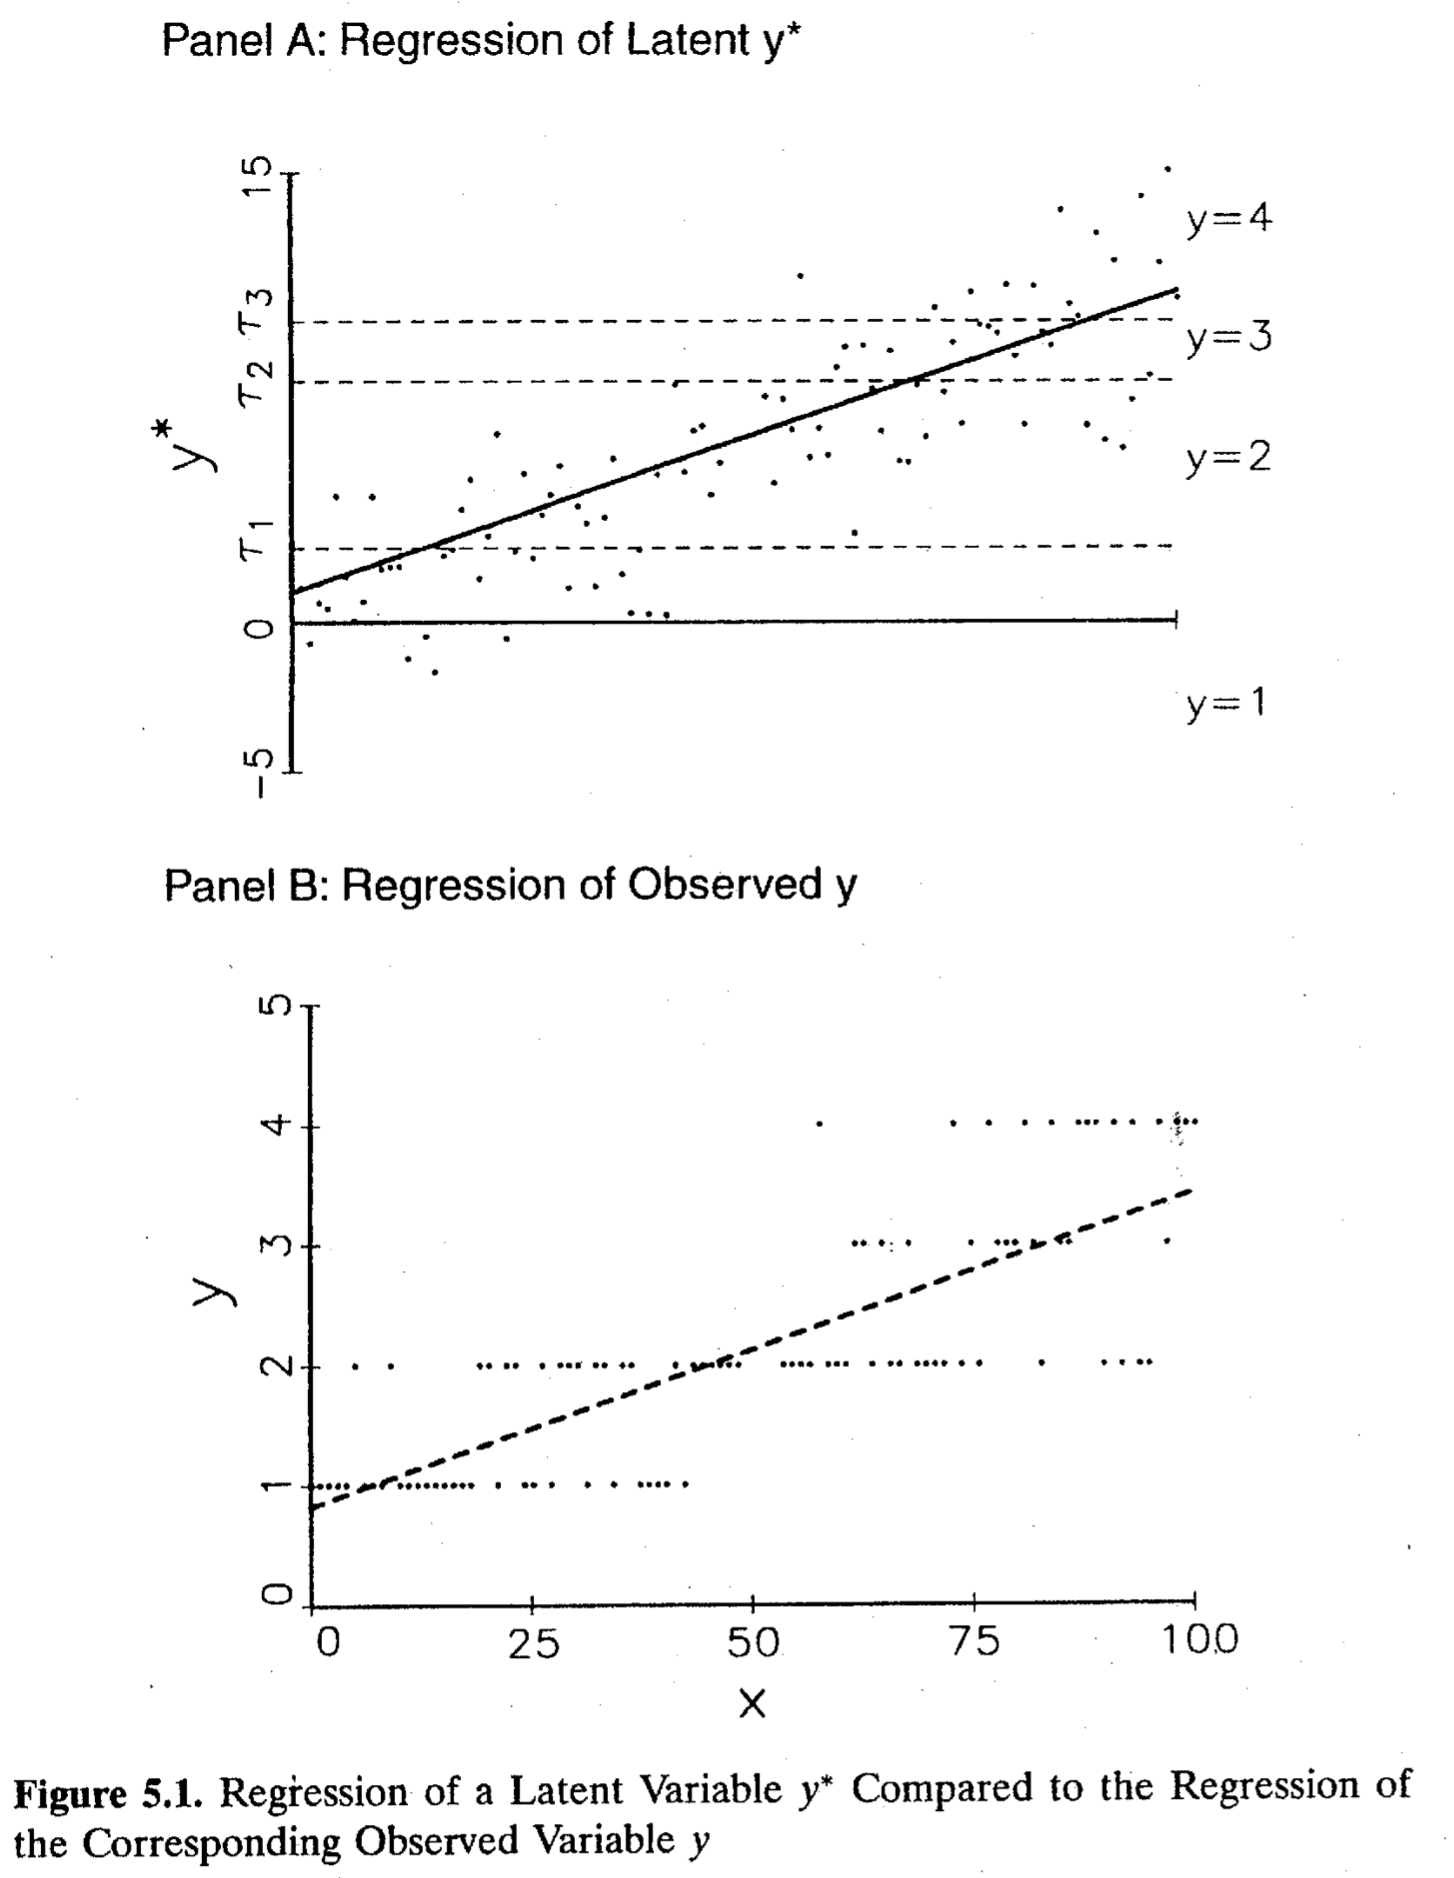
\includegraphics[width=\maxwidth]{latente_observed.png}}

Como sabemos, la estimaci\'on v\'ia modelos latentes no es posible: no podemos estimar una regresi\'on entre $y_{i}^{\star}$ y $\boldsymbol{x}$ \parencite[117]{Long:1997wv}. El otro punto que muestra la figura (en el panel inferior) es que los errores son heteroesqued\'asticos. 

\paragraph{Supuestos Distribucionales} Debido a que esta es una extensi\'on directa del modelo logit/probit, tenemos dos opciones de distribuciones, logit y probit. Como ya sabemos, {\bf estas son las distribuciones de los errores}. El PDF del modelo ordered probit es formalmente,


\begin{equation}%\label{logit.structural}
\phi(e) = \frac{1}{\sqrt{2\pi}}\text{exp}(-\frac{\epsilon^{2}}{2})
\end{equation}

donde $\phi(e) \sim (0,1)$.

El PDF del modelo ordered logit es formalmente definido como sigue,

\begin{equation}%\label{logit.structural}
\lambda(\epsilon) = \frac{\text{exp}(\epsilon)}{[1+\text{exp}(\epsilon)]^{2}}
\end{equation}

donde $\lambda(\epsilon)\sim(0, \frac{\pi^{2}}{3})$.

\paragraph{Estimacion: Probabilidades y Likelihood} Continuando con el \autoref{logit.structural}, $\boldsymbol{x_{i}}\boldsymbol{\beta} + \epsilon_{i}$ es posible de ser calculado en t\'erminos de probabilidades de la siguiente manera,


\begin{equation}%\label{logit.structural}
\text{Pr}(y_{i}=1|\boldsymbol{x_{i}}) = \text{Pr}(\tau_{0} \leq \boldsymbol{x_{i}}\boldsymbol{\beta} + \epsilon_{i} < \tau_{1}|x_{i})
\end{equation}

donde es posible de generalizar esta notaci\'on con el resto de los valores de $y_{i}$. Y asumiendo que las observaciones son independientes entre s\'i, el likelihood est\'a dado por,

\begin{equation}%\label{logit.structural}
L(\boldsymbol{\beta},\boldsymbol{\tau}|y, \boldsymbol{X}) = \prod_{i=1}^{N}\text{Pr}(y_{i})
\end{equation}

\section{Programaci\'on}

Carguemos los datos
\begin{knitrout}
\definecolor{shadecolor}{rgb}{0.969, 0.969, 0.969}\color{fgcolor}\begin{kframe}
\begin{alltt}
\hlkwd{p_load}\hlstd{(foreign)}
\hlstd{dat} \hlkwb{=} \hlkwd{read.dta}\hlstd{(}\hlstr{"https://github.com/hbahamonde/MLE/raw/master/Datasets/nes92_ordered.dta"}\hlstd{)}
\end{alltt}
\end{kframe}
\end{knitrout}

Hagamos un resumen,

\begin{knitrout}
\definecolor{shadecolor}{rgb}{0.969, 0.969, 0.969}\color{fgcolor}\begin{kframe}
\begin{alltt}
\hlkwd{summary}\hlstd{(dat)}
\end{alltt}
\begin{verbatim}
##     bushapp        ideology        bushideo      clintideo      distbushideo  
##  Min.   :0.00   Min.   :1.000   Min.   :1.00   Min.   :1.000   Min.   :0.000  
##  1st Qu.:0.00   1st Qu.:2.000   1st Qu.:4.00   1st Qu.:2.000   1st Qu.:1.000  
##  Median :1.00   Median :5.000   Median :6.00   Median :3.000   Median :2.000  
##  Mean   :1.25   Mean   :4.245   Mean   :5.15   Mean   :3.096   Mean   :2.106  
##  3rd Qu.:2.00   3rd Qu.:6.000   3rd Qu.:6.00   3rd Qu.:4.000   3rd Qu.:3.000  
##  Max.   :3.00   Max.   :7.000   Max.   :7.00   Max.   :7.000   Max.   :6.000  
##  NA's   :23     NA's   :151     NA's   :72     NA's   :84      NA's   :175    
##  distclintideo     econworse        oppforce     gulfwarworthit  
##  Min.   :0.000   Min.   :1.000   Min.   :1.000   Min.   :0.0000  
##  1st Qu.:1.000   1st Qu.:3.000   1st Qu.:3.000   1st Qu.:0.0000  
##  Median :2.000   Median :4.000   Median :3.000   Median :1.0000  
##  Mean   :2.068   Mean   :4.015   Mean   :2.964   Mean   :0.5835  
##  3rd Qu.:3.000   3rd Qu.:5.000   3rd Qu.:3.000   3rd Qu.:1.0000  
##  Max.   :6.000   Max.   :5.000   Max.   :5.000   Max.   :1.0000  
##  NA's   :190     NA's   :10      NA's   :8       NA's   :37      
##       pid            educyears        govtemp          union       
##  Min.   :-3.0000   Min.   : 2.00   Min.   :0.000   Min.   :0.0000  
##  1st Qu.:-2.0000   1st Qu.:12.00   1st Qu.:0.000   1st Qu.:0.0000  
##  Median : 0.0000   Median :13.00   Median :0.000   Median :0.0000  
##  Mean   :-0.1092   Mean   :13.57   Mean   :0.136   Mean   :0.1653  
##  3rd Qu.: 2.0000   3rd Qu.:16.00   3rd Qu.:0.000   3rd Qu.:0.0000  
##  Max.   : 3.0000   Max.   :17.00   Max.   :1.000   Max.   :1.0000  
##  NA's   :8         NA's   :5                                       
##      faminc          minority         _est_m2          _est_m1      
##  Min.   :  1.50   Min.   :0.0000   Min.   :0.0000   Min.   :0.0000  
##  1st Qu.: 21.00   1st Qu.:0.0000   1st Qu.:0.0000   1st Qu.:0.0000  
##  Median : 37.50   Median :0.0000   Median :1.0000   Median :1.0000  
##  Mean   : 41.93   Mean   :0.1347   Mean   :0.6787   Mean   :0.6787  
##  3rd Qu.: 55.00   3rd Qu.:0.0000   3rd Qu.:1.0000   3rd Qu.:1.0000  
##  Max.   :140.00   Max.   :1.0000   Max.   :1.0000   Max.   :1.0000  
##  NA's   :55
\end{verbatim}
\end{kframe}
\end{knitrout}

En esta aplicaci\'on pensaremos en la variable \texttt{econworse}: \emph{Cree usted que la economia ha empeorado?} [\texttt{Muy de acuerdo}, \texttt{de acuerdo}, \texttt{neutral}, \texttt{desacuerdo}, \texttt{muy en desacuerdo}]. Ve\'amos c\'omo se ve esta variable.

\begin{knitrout}
\definecolor{shadecolor}{rgb}{0.969, 0.969, 0.969}\color{fgcolor}\begin{kframe}
\begin{alltt}
\hlkwd{hist}\hlstd{(dat}\hlopt{$}\hlstd{econworse)}
\end{alltt}
\end{kframe}

{\centering 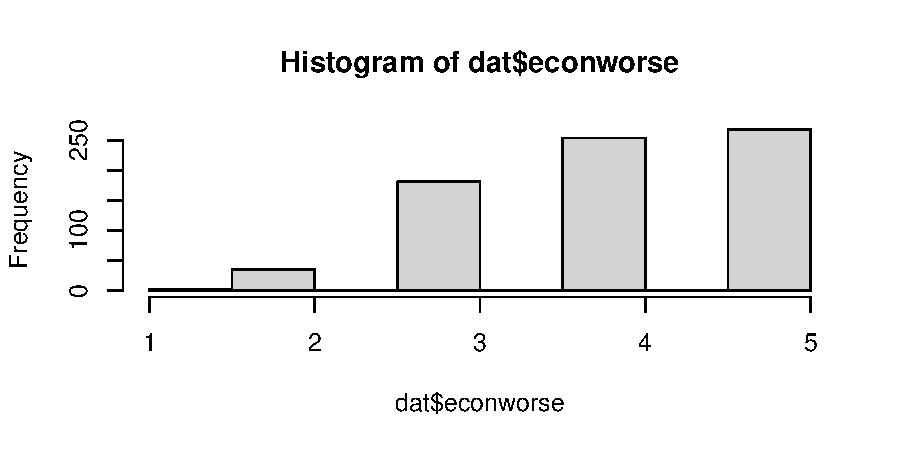
\includegraphics[width=\maxwidth]{figure/hist-1} 

}



\end{knitrout}

El paquete de \texttt{R} que usaremos se llama \texttt{polr}---\'este especifica que la variable dependiente debe ser \texttt{factor}. 

\begin{knitrout}
\definecolor{shadecolor}{rgb}{0.969, 0.969, 0.969}\color{fgcolor}\begin{kframe}
\begin{alltt}
\hlstd{dat}\hlopt{$}\hlstd{econworse.f} \hlkwb{=} \hlkwd{as.factor}\hlstd{(dat}\hlopt{$}\hlstd{econworse)} \hlcom{# transforma a factor}
\hlkwd{head}\hlstd{(dat}\hlopt{$}\hlstd{econworse.f)} \hlcom{# ve como queda}
\end{alltt}
\begin{verbatim}
## [1] 4 5 5 5 4 5
## Levels: 1 2 3 4 5
\end{verbatim}
\end{kframe}
\end{knitrout}

Ahora estimemos un \texttt{ologit} y un \texttt{oprobit}.

\begin{knitrout}
\definecolor{shadecolor}{rgb}{0.969, 0.969, 0.969}\color{fgcolor}\begin{kframe}
\begin{alltt}
\hlkwd{p_load}\hlstd{(MASS)}
\hlstd{o.logit} \hlkwb{=} \hlkwd{polr}\hlstd{(econworse.f} \hlopt{~} \hlstd{ideology} \hlopt{+} \hlstd{educyears} \hlopt{+} \hlstd{faminc,} \hlkwc{data} \hlstd{= dat,}  \hlkwc{method} \hlstd{=} \hlstr{"logistic"}\hlstd{)} \hlcom{# o-logit}
\hlstd{o.probit} \hlkwb{=} \hlkwd{polr}\hlstd{(econworse.f} \hlopt{~} \hlstd{ideology} \hlopt{+} \hlstd{educyears} \hlopt{+} \hlstd{faminc,} \hlkwc{data} \hlstd{= dat,}  \hlkwc{method} \hlstd{=} \hlstr{"probit"}\hlstd{)} \hlcom{# o-probit}
\end{alltt}
\end{kframe}
\end{knitrout}

Desde ahora en adelante, prestaremos m\'as atenci\'on a la presentaci\'on de resultados. Hagamos una tabla.

\begin{kframe}
\begin{alltt}
\hlkwd{p_load}\hlstd{(texreg)}
\hlkwd{texreg}\hlstd{(}\hlkwd{list}\hlstd{(o.logit, o.probit))} \hlcom{# usa "screenreg" no "texreg".}
\end{alltt}
\end{kframe}
\begin{table}
\begin{center}
\begin{tabular}{l c c}
\hline
 & Model 1 & Model 2 \\
\hline
ideology       & $-0.27^{***}$ & $-0.17^{***}$ \\
               & $(0.05)$      & $(0.03)$      \\
educyears      & $-0.09^{*}$   & $-0.06^{*}$   \\
               & $(0.04)$      & $(0.02)$      \\
faminc         & $-0.00$       & $-0.00$       \\
               & $(0.00)$      & $(0.00)$      \\
1|2            & $-8.97^{***}$ & $-4.63^{***}$ \\
               & $(1.16)$      & $(0.48)$      \\
2|3            & $-5.57^{***}$ & $-3.27^{***}$ \\
               & $(0.62)$      & $(0.35)$      \\
3|4            & $-3.44^{***}$ & $-2.11^{***}$ \\
               & $(0.58)$      & $(0.33)$      \\
4|5            & $-1.91^{***}$ & $-1.17^{***}$ \\
               & $(0.57)$      & $(0.33)$      \\
\hline
AIC            & $1353.41$     & $1350.17$     \\
BIC            & $1383.68$     & $1380.44$     \\
Log Likelihood & $-669.70$     & $-668.09$     \\
Deviance       & $1339.41$     & $1336.17$     \\
Num. obs.      & $558$         & $558$         \\
\hline
\multicolumn{3}{l}{\scriptsize{$^{***}p<0.001$; $^{**}p<0.01$; $^{*}p<0.05$}}
\end{tabular}
\caption{Statistical models}
\label{table:coefficients}
\end{center}
\end{table}


Ya que los resultados son (casi) siempre similares, durante el resto de la clase solo veremos el \texttt{o.logit}.

F\'ijate que vemos mas interceptos, uno por cada $\tau$. Debido a que $y_{i}$ tiene cinco valores, hay cuatro $\tau$. Esto se puede interpretar as\'i,

\begin{equation}\label{logit.inter}
\begin{split}
\text{logit}(Pr(y_{i}\leq1)) = -8.97 -0.27\times\text{\texttt{ideology}}_{i} -0.09\times\text{\texttt{educyears}}_{i} - 0\times\text{\texttt{faminc}}_{i} \\
\text{logit}(Pr(y_{i}\leq2)) = -5.57 -0.27\times\text{\texttt{ideology}}_{i} -0.09\times\text{\texttt{educyears}}_{i} - 0\times\text{\texttt{faminc}}_{i} \\
\text{logit}(Pr(y_{i}\leq3)) = -3.44 -0.27\times\text{\texttt{ideology}}_{i} -0.09\times\text{\texttt{educyears}}_{i} - 0\times\text{\texttt{faminc}}_{i} \\
\text{logit}(Pr(y_{i}\leq4)) = -1.91 -0.27\times\text{\texttt{ideology}}_{i} -0.09\times\text{\texttt{educyears}}_{i} - 0\times\text{\texttt{faminc}}_{i} 
\end{split}
\end{equation}

\section{Interpretaci\'on} 

Ahora interpretaremos el modelo. 

\paragraph{Intervalos de Confianza} Inspeccionemos los intervalos de confianza,

\begin{knitrout}
\definecolor{shadecolor}{rgb}{0.969, 0.969, 0.969}\color{fgcolor}\begin{kframe}
\begin{alltt}
\hlkwd{p_load}\hlstd{(coefplot)}
\hlkwd{coefplot}\hlstd{(o.logit)}
\end{alltt}
\end{kframe}

{\centering 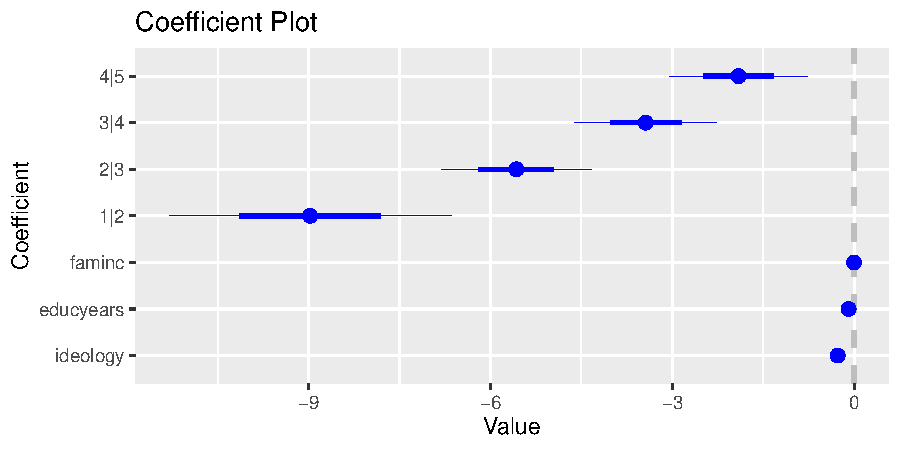
\includegraphics[width=\maxwidth]{figure/coefplot-1} 

}



\end{knitrout}

El eje $x$ del gr\'afico est\'a en escala de logit, o \emph{log-odds}. Es decir, si subo una unidad en \texttt{ideology}, esperamos que \texttt{econworse.f} suba  -0.27 {\bf en la escala logit, o log-odds} manteniendo las otras variables constantes en sus medias. 

\paragraph{Odds Ratios} Calculemos ahora los \emph{odds ratios}.


\begin{knitrout}
\definecolor{shadecolor}{rgb}{0.969, 0.969, 0.969}\color{fgcolor}\begin{kframe}
\begin{alltt}
\hlkwd{exp}\hlstd{(}\hlkwd{coef}\hlstd{(o.logit))}
\end{alltt}
\begin{verbatim}
##  ideology educyears    faminc 
## 0.7622486 0.9131977 0.9977306
\end{verbatim}
\end{kframe}
\end{knitrout}

Esto quiere decir que cuando subo una unidad en \texttt{ideology} (i.e. me vuelvo mas derechista) es 0.76 m\'as \emph{posible} que encuentre la econom\'ia peor (\texttt{econworse}), manteniendo el resto de las variables constantes en sus medias. El supuesto que permite esta comparacion, i.e. de que los odds ratios se aplican a cualquier nivel de la $y_{i}$, se llama {\bf parallel regression assumption} \parencite[140]{Long:1997wv}. Por esto es que estos \emph{odds ratios} son \emph{proporcionales} (aplican en cualquier intervalo de \texttt{ideology}). Este supuesto es testable v\'ia el \emph{Brant test}.

\begin{knitrout}
\definecolor{shadecolor}{rgb}{0.969, 0.969, 0.969}\color{fgcolor}\begin{kframe}
\begin{alltt}
\hlkwd{p_load}\hlstd{(brant)}
\hlkwd{brant}\hlstd{(o.logit)}
\end{alltt}
\begin{verbatim}
## -------------------------------------------- 
## Test for	X2	df	probability 
## -------------------------------------------- 
## Omnibus		7.22	9	0.61
## ideology	4.74	3	0.19
## educyears	2.43	3	0.49
## faminc		1.25	3	0.74
## -------------------------------------------- 
## 
## H0: Parallel Regression Assumption holds
\end{verbatim}
\end{kframe}
\end{knitrout}

La $H_{0}$ es que se cumple el supuesto de la regresi\'on paralela. Si la probabilidad de la $H_{1}$ (que aparece en la tabla) es ``alta'', el supuesto---probablemente---no se cumple.

\paragraph{Cambios Marginales} Calculemos ahora los cambios marginales. Pensemos en dos perfiles.


\begin{knitrout}
\definecolor{shadecolor}{rgb}{0.969, 0.969, 0.969}\color{fgcolor}\begin{kframe}
\begin{alltt}
\hlkwd{p_load}\hlstd{(margins)}
\hlcom{# 1}
\hlkwd{margins}\hlstd{(o.logit,} \hlkwc{at} \hlstd{=} \hlkwd{list}\hlstd{(}
  \hlkwc{ideology} \hlstd{=} \hlkwd{max}\hlstd{(dat}\hlopt{$}\hlstd{ideology,} \hlkwc{na.rm} \hlstd{= T),} \hlcom{# derechista }
  \hlkwc{educyears} \hlstd{=} \hlkwd{min}\hlstd{(dat}\hlopt{$}\hlstd{educyears,} \hlkwc{na.rm} \hlstd{= T))} \hlcom{# sin educ}
  \hlstd{)}
\end{alltt}
\begin{verbatim}
##  at(ideology) at(educyears)  ideology educyears      faminc
##             7             2 0.0003049  0.000102 0.000002552
\end{verbatim}
\begin{alltt}
\hlcom{# 2}
\hlkwd{margins}\hlstd{(o.logit,} \hlkwc{at} \hlstd{=} \hlkwd{list}\hlstd{(}
  \hlkwc{ideology} \hlstd{=} \hlkwd{min}\hlstd{(dat}\hlopt{$}\hlstd{ideology,} \hlkwc{na.rm} \hlstd{= T),} \hlcom{# izquierdista}
  \hlkwc{educyears} \hlstd{=} \hlkwd{min}\hlstd{(dat}\hlopt{$}\hlstd{educyears,} \hlkwc{na.rm} \hlstd{= T))} \hlcom{# sin educ}
\hlstd{)}
\end{alltt}
\begin{verbatim}
##  at(ideology) at(educyears)   ideology  educyears       faminc
##             1             2 0.00005992 0.00002004 0.0000005014
\end{verbatim}
\end{kframe}
\end{knitrout}


\paragraph{Predicted probabilities} Calculemos ahora los \emph{predicted probabilities}. 

\begin{knitrout}
\definecolor{shadecolor}{rgb}{0.969, 0.969, 0.969}\color{fgcolor}\begin{kframe}
\begin{alltt}
\hlkwd{p_load}\hlstd{(effects)}
\hlkwd{plot}\hlstd{(}\hlkwd{effect}\hlstd{(}\hlstr{"ideology"}\hlstd{, o.logit))}
\end{alltt}
\end{kframe}

{\centering 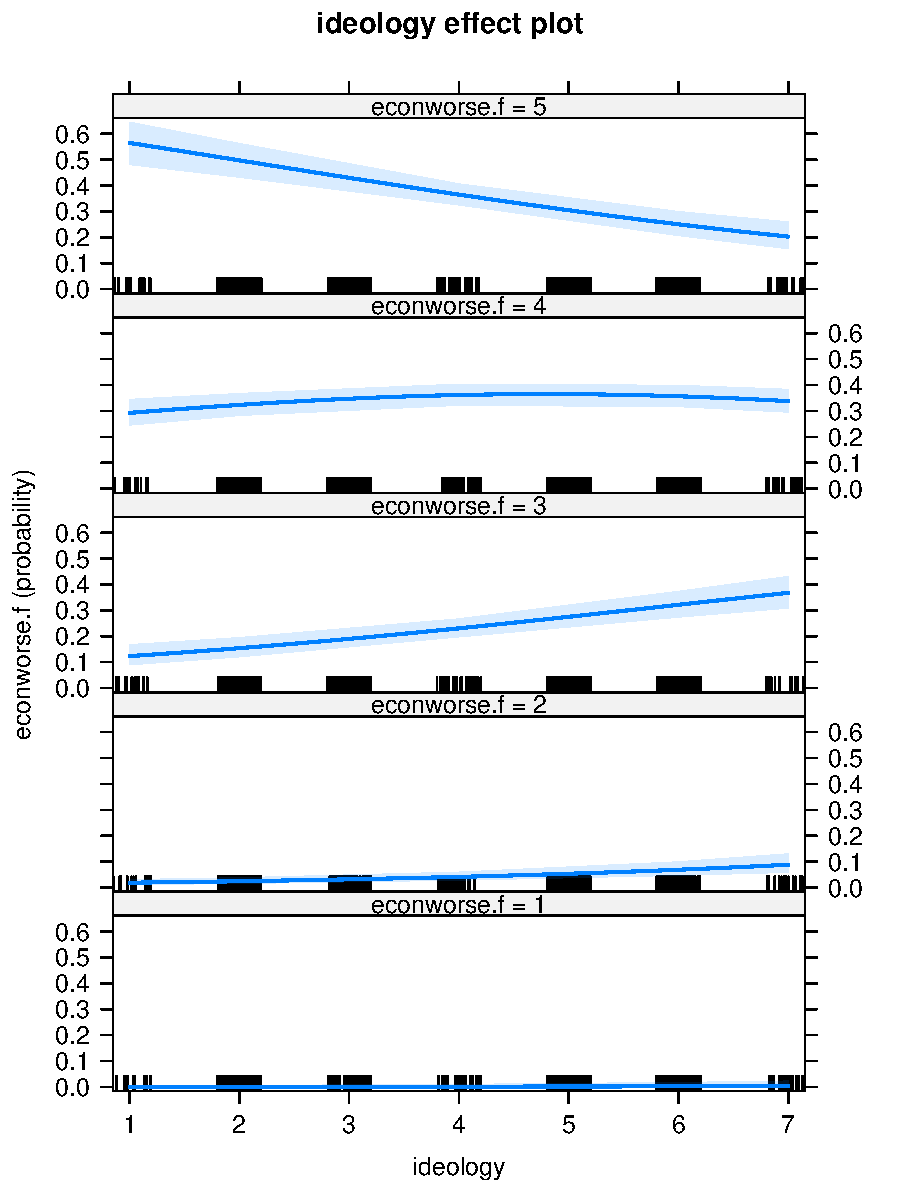
\includegraphics[width=\maxwidth]{figure/pp-1} 

}


\begin{kframe}\begin{alltt}
\hlkwd{plot}\hlstd{(}\hlkwd{effect}\hlstd{(}\hlstr{"educyears"}\hlstd{, o.logit))}
\end{alltt}
\end{kframe}

{\centering 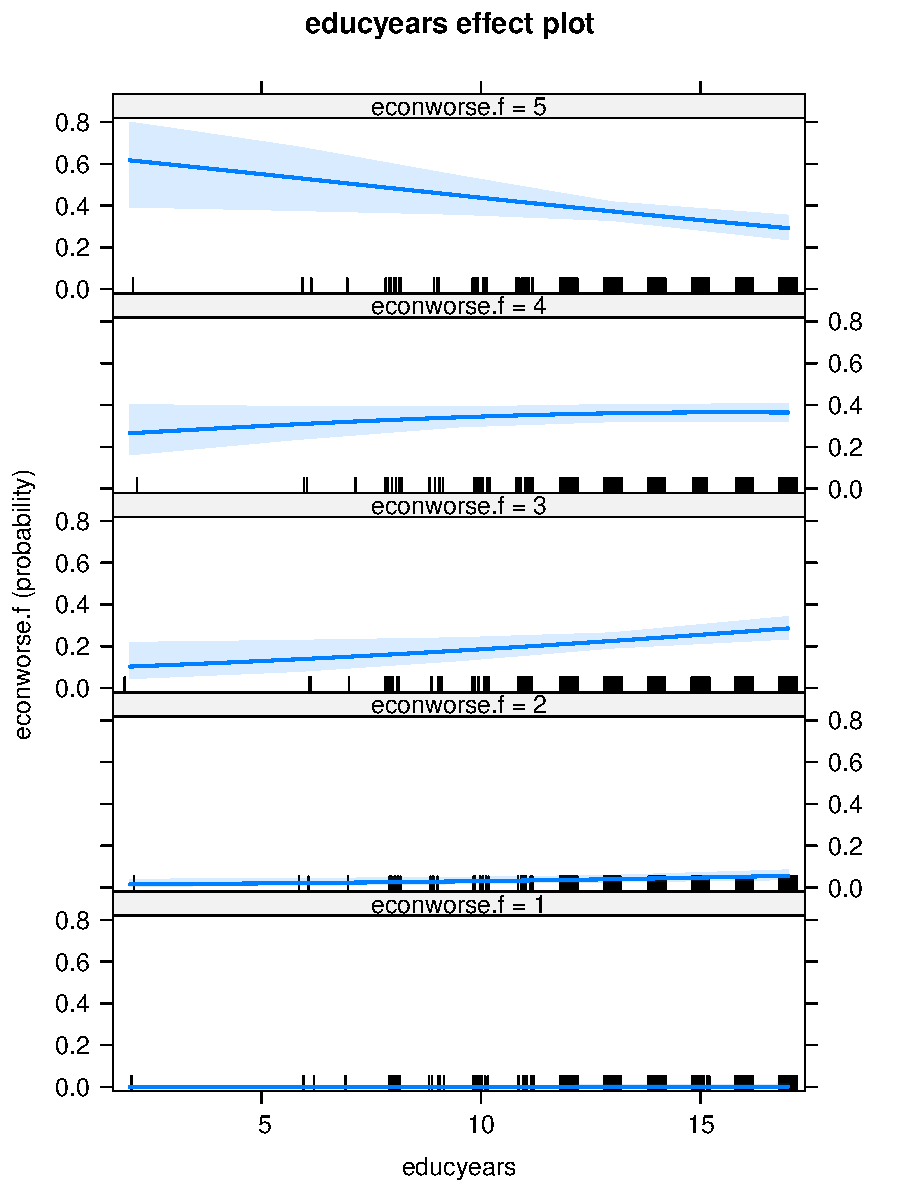
\includegraphics[width=\maxwidth]{figure/pp-2} 

}


\begin{kframe}\begin{alltt}
\hlkwd{plot}\hlstd{(}\hlkwd{effect}\hlstd{(}\hlstr{"faminc"}\hlstd{, o.logit))}
\end{alltt}
\end{kframe}

{\centering 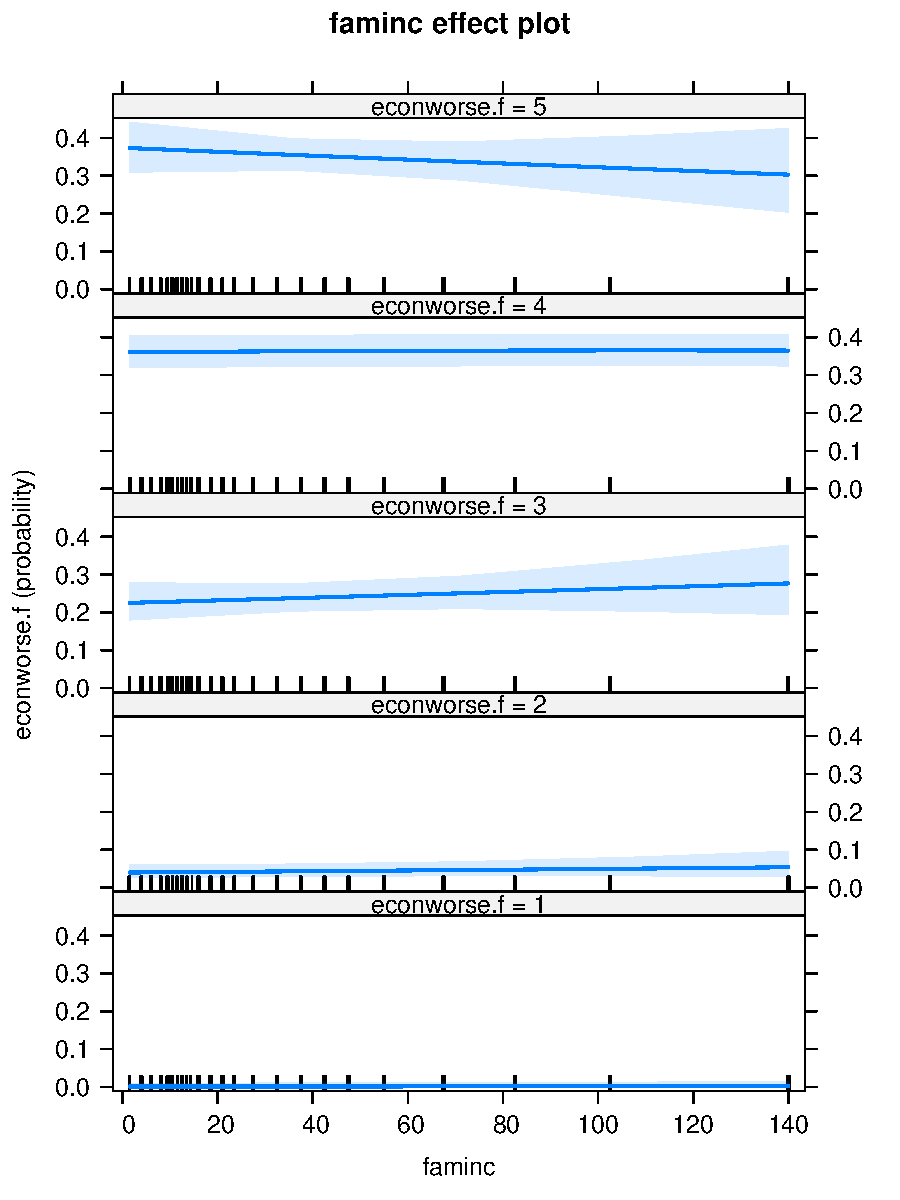
\includegraphics[width=\maxwidth]{figure/pp-3} 

}



\end{knitrout}

\begin{knitrout}
\definecolor{shadecolor}{rgb}{0.969, 0.969, 0.969}\color{fgcolor}\begin{kframe}
\begin{alltt}
\hlstd{knitr}\hlopt{::}\hlkwd{purl}\hlstd{(}\hlstr{'Ordered.Rnw'}\hlstd{)}
\end{alltt}


{\ttfamily\noindent\bfseries\color{errorcolor}{\#\# Error in parse\_block(g[-1], g[1], params.src, markdown\_mode): Duplicate chunk label 'setup', which has been used for the chunk:\\\#\# if (!require("{}pacman"{})) install.packages("{}pacman"{}); library(pacman)\\\#\# p\_load(knitr)\\\#\# set.seed(2020)\\\#\# options(scipen=9999999)}}\begin{alltt}
\hlkwd{Stangle}\hlstd{(}\hlstr{'Ordered.Rnw'}\hlstd{)}
\end{alltt}
\begin{verbatim}
## Writing to file Ordered.R
\end{verbatim}


{\ttfamily\noindent\bfseries\color{errorcolor}{\#\# Error in match.arg(options\$results, c("{}verbatim"{}, "{}tex"{}, "{}hide"{})): 'arg' should be one of "{}verbatim"{}, "{}tex"{}, "{}hide"{}}}\end{kframe}
\end{knitrout}




%\newpage
%\paragraph{}
%\paragraph{}
%\pagenumbering{Roman}
%\setcounter{page}{1}
%\printbibliography



\end{document}


